\chapter{Dinâmica de Opinião} %#{{{1

%#{{{

Nos últimos anos é crescente o interesse em modelagem física de
sociedades. Em 2009, foi publicado um \textit{Review of Mordern Physics}
compilando alguns dos mais recentes avanços da pesquisa nessa área
\cited{Castellano2009}. A compreensão dos mecanismos que levam a formação
de \textbf{consenso} e \textbf{dissenso} em sociedades é uma das atuais
áreas de interesse na pesquisa de dinâmica social.  A ideia é determinar
quando a dinâmica de uma sociedade de agentes interagentes, que podem
escolher entre diferentes opções (por exemplo, opinião contra ou a favor
determinado assunto, características culturais, etc) chegará ao consenso,
i.e. a maior parte da sociedade partilhará a mesma opinião, ou a estados com
dissenso. Também é de interesse, no caso em que existe localização espacial
dos agentes, encontrar dinâmicas que levam a estados \textbf{polarizados},
ou seja, estados em que o consenso é apenas local.

Na literatura da área, existem duas principais vertentes de modelos
de agentes.  A mais estudada é a de modelos de agentes com opiniões
discretas. Na maioria, são modelos do tipo Ising onde só existem dois
tipos de opinião. A outra vertente são modelos com opinião contínua,
entre os quais podemos destacar os de modelos de agentes com o conceito de
\textit{confiança limitada} (\textit{bounded confidence}) onde os agentes
só interagem se eles tiverem a diferença de suas opiniões dentro de um
certo limite \citep{Deffuant2000, Hegselmann2002, Lorenz2007}.

Do primeiro grupo, dois exemplos de modelos conhecidos são o modelo
do \textit{Votante} \cite{Holley1975a}, e modelo de \textit{Sznajd}
\cite{Sznajd2000}. Neles, os agentes são representados por uma variável
binária $s= \pm 1$ e apresentam uma dinâmica simples. No caso do
modelo do votante, a cada passo da dinâmica um agente $i$ escolhido
aleatoriamente assume a opinião de um de seus vizinhos, também escolhido
aleatoriamente. Já na dinâmica do modelo de Sznajd um par de vizinhos é
escolhido ao acaso. Caso eles apresentem a mesma opinião, esse par irá
impor essa opinião para seus vizinhos em comum. No entanto, se esse par
tiver opiniões diferentes, cada agente irá impor sua opinião ao vizinhos do
outro agente.  Outro modelo de opiniões discreta é o modelo da \textit{Regra
da Maioria} \cite{Galam1986}. Nesse modelo, os agentes também apresentam
opiniões binárias. A dinâmica do modelo se inicia com uma fração $p_+$
de agentes de opinião $+1$ e uma $ p_- = 1 - p_+$ de opinião $-1$. A cada
passo da dinâmica, um grupo de $r$ agentes é escolhido aleatoriamente
como um grupo de discussão. O resultado da discussão será que todos os
agentes do grupo assumirão a opinião majoritária. O tamanho do grupo $r$
é sorteado aleatoriamente a cada passo da dinâmica. Além disso, se $r$
for ímpar sempre existirá uma maioria, no entanto, se $r$ for par no caso
da metade dos agentes do grupo apresentarem uma opinião diferente da outra
metade, o grupo todo será enviesado em $+1$ sem perda de generalidade.

Uma importante característica desses modelos é que suas dinâmicas levam
a estados de consenso além de serem equivalentes a processos de Monte
Carlo com temperatura nula. Eles foram estudados sobre diversos contextos,
sendo aplicados a áreas que vão além de dinâmica social. Foram feitos
estudos sobre suas convergências para diversos grafos, além de existirem
generalizações com mais de duas opiniões \citep{Castellano2009}. Apesar
de serem interessantes do ponto de vista de problemas de dinâmicas
probabilísticas, esses modelos apresentam pouca fundamentação experimental,
sendo construídos a partir de ideias muito gerais. Alguns dos problemas que
esses modelos apresentam são a falta de memória de seus agentes, e no caso
de modelos discretos, a impossibilidade de se medir o grau de similaridade
entre dois indivíduos. Afim de solucionar esses problemas, foram sugeridos
na literatura modelos de \textit{agentes brownianos} \cite{Schweitzer2000}
onde cada agente apresenta uma energia interna que é usada para influenciar
o seu comportamento futuro. Outra abordagem é o modelo opinião contínua
e ação discreta (\textit{CODA}) \cite{Martins2008}, nesse modelo, o
agente acredita em uma das duas opções possíveis com uma probabilidade
que evolui no tempo de acordo com a regra de Bayes. O consenso da sociedade
ocorre somente em nível local, aparecendo opiniões extremas e divergentes,
caracterizando um estado polarizado.

Outra característica importante não considerada nos modelos de opinião
binária é que pessoas discutem diversos assuntos simultaneamente,
sendo muito deles não passíveis de representação por um único
número. Para tanto, em 1997, Axelrod propôs um modelo de disseminação
de cultura \cite{Axelrod1997}  bastante influente tanto na física quanto na
sociologia. Seu modelo é uma generalização natural de modelos de dinâmica
de opiniões com várias dimensões. Além disso, esse modelo incorpora os
conceitos de \textit{influência social} e \textit{homofilia} que são duas
características tidas como fundamentais entre os cientistas sociais para
o entendimento da disseminação de cultura. A primeira, com explicamos
na sessão \ref{sec:pressao}, é a tendência de indivíduos se tornarem
mais similares quando interagem e a segunda é a tendência de indivíduos
parecidos interagirem mais frequentemente.

Mais especificamente, os agentes são definidos por um conjunto de números
inteiros e tamanho $F$  , $(\sigma_1,\ldots,\sigma_F)$. Cada componente
representa uma \textit{característica cultural}(\textit{features}), e cada
característica pode assumir $q$ valores, $\sigma_f = 0,1,\ldots,q-1$. Os
agentes estão situados sobre os nós de um grafo que pode ser regular
ou não, e inicialmente suas características são sorteadas aleatoriamente. Na
dinâmica do modelo, a cada passo de tempo, um agente $i$ e um vizinho $j$ são
sorteados. A probabilidade desses dois agentes interagirem é dada pela média
de características $\omega_{ij}$ comuns entre eles, que é definido por,
\[
\omega_{ij} = \frac{1}{F} \sum_{f=1}^F \delta_{\sigma_f^i\sigma_f^j}
\]
onde $\delta_{\sigma^i\sigma^j}$ é o delta de Kronecker.  Na interação o
agente $j$ assume uma características do agente $i$ que não é comum entre
eles: $\sigma_f^j(t+1)=\sigma_f^i(t)$ se $\sigma_f^j(t)\neq\sigma_f^i(t)$. Os
conceitos de homofilia e influência social são usados no modelo, pois quanto
mais similares são os agentes maior a probabilidade deles interagirem e a
interação entre os agentes os deixam mais parecidos. A dinâmica do modelo
de Axelrod é bastante rica, para um número pequeno de características é
possível encontrar estados estacionários de consenso, no entanto, quando o
número de características cresce o estado estacionário é de total dissenso.
%#}}}

\section{Sociedade de Perceptrons} %#{{{2
\label{sec:plandia}

Nessa sessão é descrito o modelo proposto em \citep{Caticha2011a} e que
serviu de base para o trabalho principal apresentado na tese. Enfatizamos
algumas propriedades desse modelo obtidas através de cálculos
numéricos. Sobre o contexto de redes neurais, podemos dizer que os agentes
do modelo são perceptrons com vetores sinápticos $\bm{\omega}_i \in \Re^N
$, onde $i=1, 2,\ldots,K$  é o índice do agente e $K$ é número total de
agentes na sociedade. A interação entre os agentes se dá pela discussão
de assuntos públicos representados pelos vetores $\bm{x}_\mu$ sendo $\mu$
um índice temporal. A cada passo $\mu$ da dinâmica, uma dupla de agentes
vizinho $\bm{\omega}_i$ e $\bm{\omega}_j$ é escolhida aleatoriamente para
discutir um assunto $\bm{x}_\mu$ e com probabilidade $1/2$ um dos agentes é
sorteado para ser o aluno enquanto o outro agente será o professor. Portanto,
para cada interação um dos vizinhos tenta aprender a direção do outro
usando o algoritmo da equação \eqref{eq:Japrende},
\begin{align}
    \bm{\omega}_i^\prime&= \bm{\omega}_i^\mu - 
        \frac{1}{N}\nabla_{\bm{\omega}_i} H +\bm{\eta}, \nn
    &= \bm{\omega}_i^\mu + \frac{1}{N}\sigma_j^\mu\bm{x}_\mu F_\delta
        + \bm{\eta}.
\label{eq:Japrende}
\end{align} 

Onde $H\left(\left\{\bm{\omega}_j\right\}_{j=1,\ldots,K},\bm{x}\right)$
é a Hamiltoniana do sistema e $F_\delta = - \nabla_{\bm{\omega}_i}
H $ é a função de modulação do aprendizado e $\sigma_j^\mu =
sign\left(\bm{\omega}_j^\mu\cdot\bm{x}_\mu\right)$ é a classificação dada
pelo agente $j$ sobre o assunto que é discutido no tempo $\mu$. O termo
$\bm{\eta}$ é um ruído gaussiano com média nula e pretende descrever uma
falha de comunicação entre os agentes. Vamos impor que o vetores sinápticos
dos agentes sejam sempre normalizados para impedir que existam agentes com
opiniões muito mais relevantes que de outros na sociedade:
\[
\tilde{\bm{\omega}}_i = \frac{\bm \omega_i^\prime}
                {\left|\bm \omega_i^\prime\right|}.
\]
Para um ruído gaussiano com variância suficientemente grande, podemos
fazer uma dinâmica de Metropolis para a evolução da sociedade. Impondo
a condição de balanceamento detalhado para a interação entre os
agentes, o agente $i$ aceitará a mudança nos seus pesos sinápticos ($
\bm{\omega}_i^{\mu + 1} = \tilde{\bm{\omega}}_i $) se isso diminuir a energia
de interação com a sua vizinhança, caso contrário ele mudará seus pesos
sinápticos com uma probabilidade $p$ dada por,
\begin{equation}
p = e^{-\alpha\left( H_{\left( new \right)} - H_{\left( old \right)} \right)},
\end{equation}  
onde $\alpha$ é denominado de pressão de pares e é usualmente interpretado
como o inverso da temperatura do sistema em outros modelos de Mecânica
Estatística \footnote{No texto principal chamamos o termo de pressão de
pares de $\beta$ ao invés de $\alpha$.}.

A Hamiltoniana que rege a dinâmica da sociedade deverá ser construída como a
somatória do potencial de interação entre os pares,  
\begin{equation}
H = \sum_{\left(i,j\right)}  
    V\left(\bm{\omega}_i^\mu,\bm{\omega}_j^\mu,\bm{x}_\mu\right),
\label{eq:H1} 
\end{equation}
onde $(i,j)$ representa a soma sobre primeiros vizinhos. A vizinhança da
sociedade é definida através de um grafo $\mathcal{G}$ que pode ser tanto
uma rede regular quanto um grafo com distribuição de arestas aleatória.

Assim como foi feito no texto principal, estudamos a dinâmica de opinião
da sociedade no caso em que os agentes discutem um único assunto, chamado
\textit{Zeitgeist}, em todos os passos da dinâmica, ou seja, $\bm{x}_\mu =
\mc Z$ para todo $\mu$, sendo que $\left|\mc Z\right| = 1$.

O potencial de interação entre dois agentes na sociedade que foi introduzido
por Caticha e Renato\citep{Caticha2011a} é,
\begin{equation}
V \left(\bm{\omega}_i,\bm{\omega}_j,\mc Z\right)= 
    -\frac{1 + \delta }{2}h_ih_j +\frac{ 1 -\delta}{2}|h_i||h_j|.
\label{eq:Vdelta1}
\end{equation}
onde $h_i^\mu = \bm{\omega}_i^\mu \cdot \bm{x}_\mu $  é  a
\textit{sobreposição} entre o vetor sináptico do agente $i$ e
\textit{Zeitgeist} ou simplesmente a \textit{opinião} do agente em relação
ao \textit{Zeitgeist}.  Já a função de modulação que rege o aprendizado
dos agentes no modelo é definida por
\begin{equation}
W_{i}^\mu = W_{\delta}^\mu 
= 1 -\left( 1- \delta\right)\Theta\left(-h_i^\mu\sigma_j^\mu\right).
\label{eq:W1}
\end{equation}

\begin{figure}
    \centering
    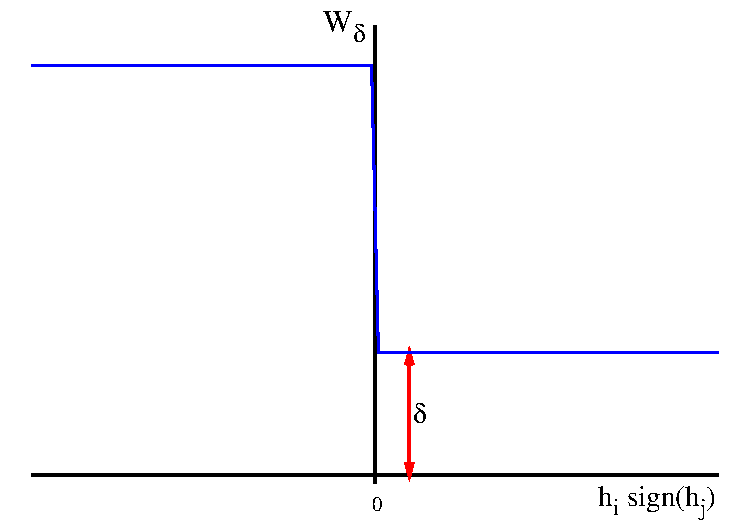
\includegraphics[width=0.5\textwidth]{Figures/fdelta}
    \caption{
      Função de Modulação. O parâmetro $\delta$ representa a tendência
      que o agente tem de entrar em conformidade, ou seja, quanto maior for
      o valor de $\delta$ mais o agente irá aprender com um assunto que
      ele é concordante.  Analogamente, podemos interpretar $1 - \delta$ como a
      grau de importância a novidade.
  } 
  \label{fig:fdelta}
\end{figure}

Podemos perceber mais claramente através da figura \ref{fig:fdelta}
que o parâmetro $\delta$ do modelo pode ser interpretado como uma tendência
corroborativa dos agentes, pois mede a tendência do agente a mudar a direção
do seu vetor sináptico quando ele está em concordância com seu parceiro
social. A grandeza $1 -\delta$ é interpretado como a importância que o agente
dá a assuntos discordantes quando comparados com assuntos em que existe
concordância com seus parceiros sociais.  Essa interpretação também pode
ser feita analisando a figura \ref{fig:Vd} onde é apresentado o potencial de
interação entre dois agentes para diferentes valores de $\delta$.em função
de $\theta_i$ e $\theta_j$, com $h_{i,j} = \cos \theta_{i,j}$.  É interessante
notar que  quando $\delta = 1$ essa função de modulação é idêntica a de
Hebb e quando $\delta = 0$ ela é igual a função do perceptron de Rosemblatt.

\begin{figure*} 
\caption{ 
    \textbf{Potencial de interação entre os agentes}  para diferentes
    valores de $\delta$ em função de $\theta_i$ e $\theta_j$, onde $h_{i,j}
    = \cos \theta_{i,j}$. 
    %Vemos que para $\delta = 0$ os agentes só interagem
    %se estiverem em concordância com o assunto, enquanto para $\delta = 1$
    %temos que a interação entre os agentes é simétrica em relação ao sinal
    %da opinião sobre o assunto, já para $\delta=0.5$ a interação entre os
    %agentes no caso em que existe discordância é intermediária em relação
    %as duas situações anteriores.
}
\centering
\begin{subfigure}{.31\textwidth }
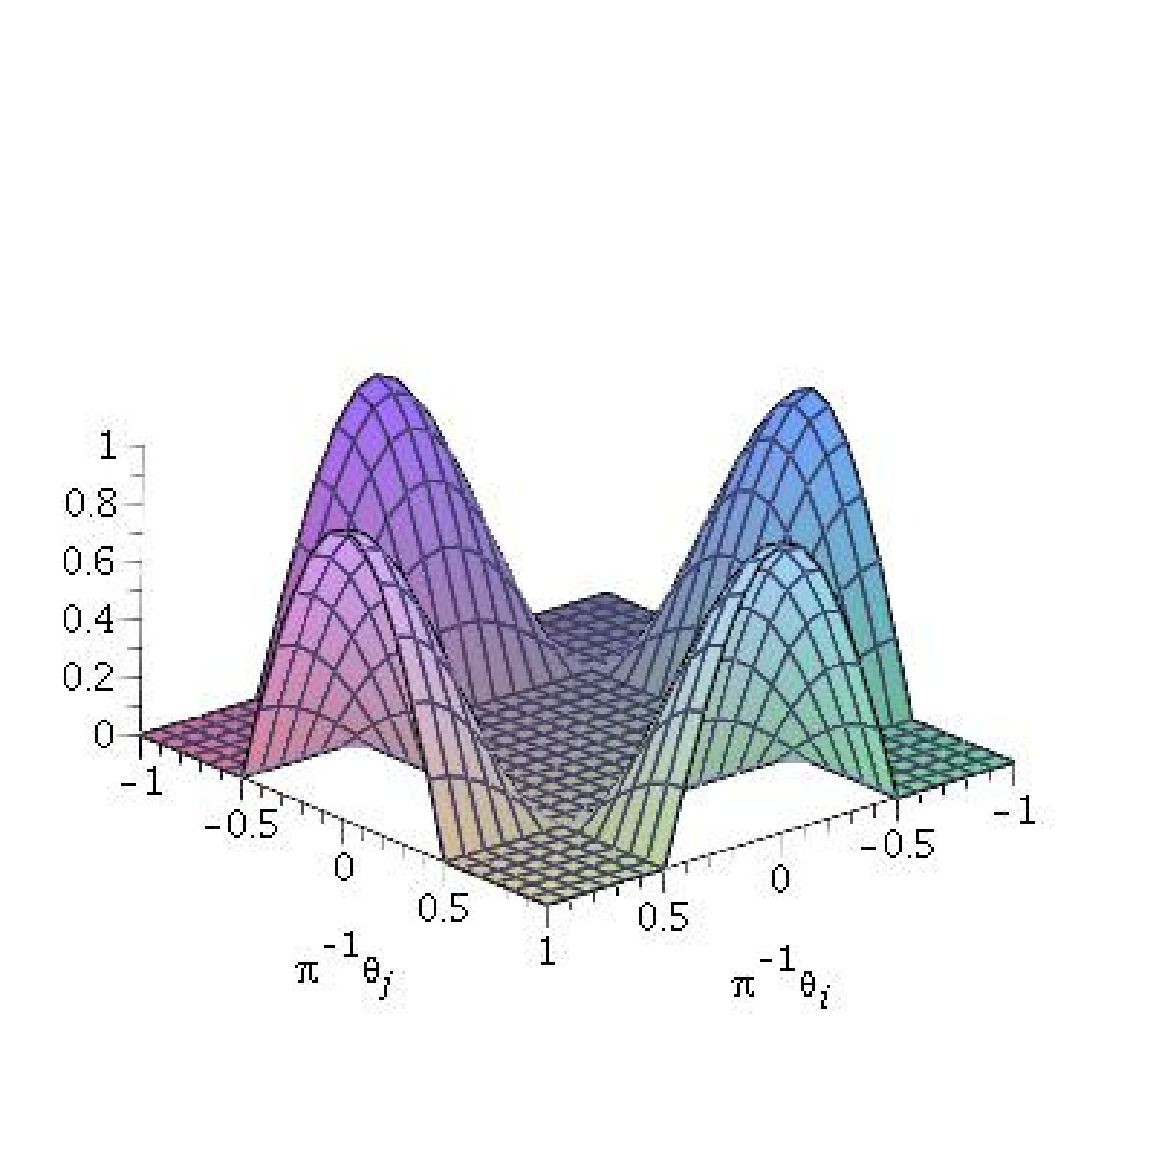
\includegraphics[width=\textwidth]{Figures/Vd0}
\caption{ $\delta = 0.0$}
\end{subfigure}
%
\begin{subfigure}{0.31\textwidth }
    \centering
    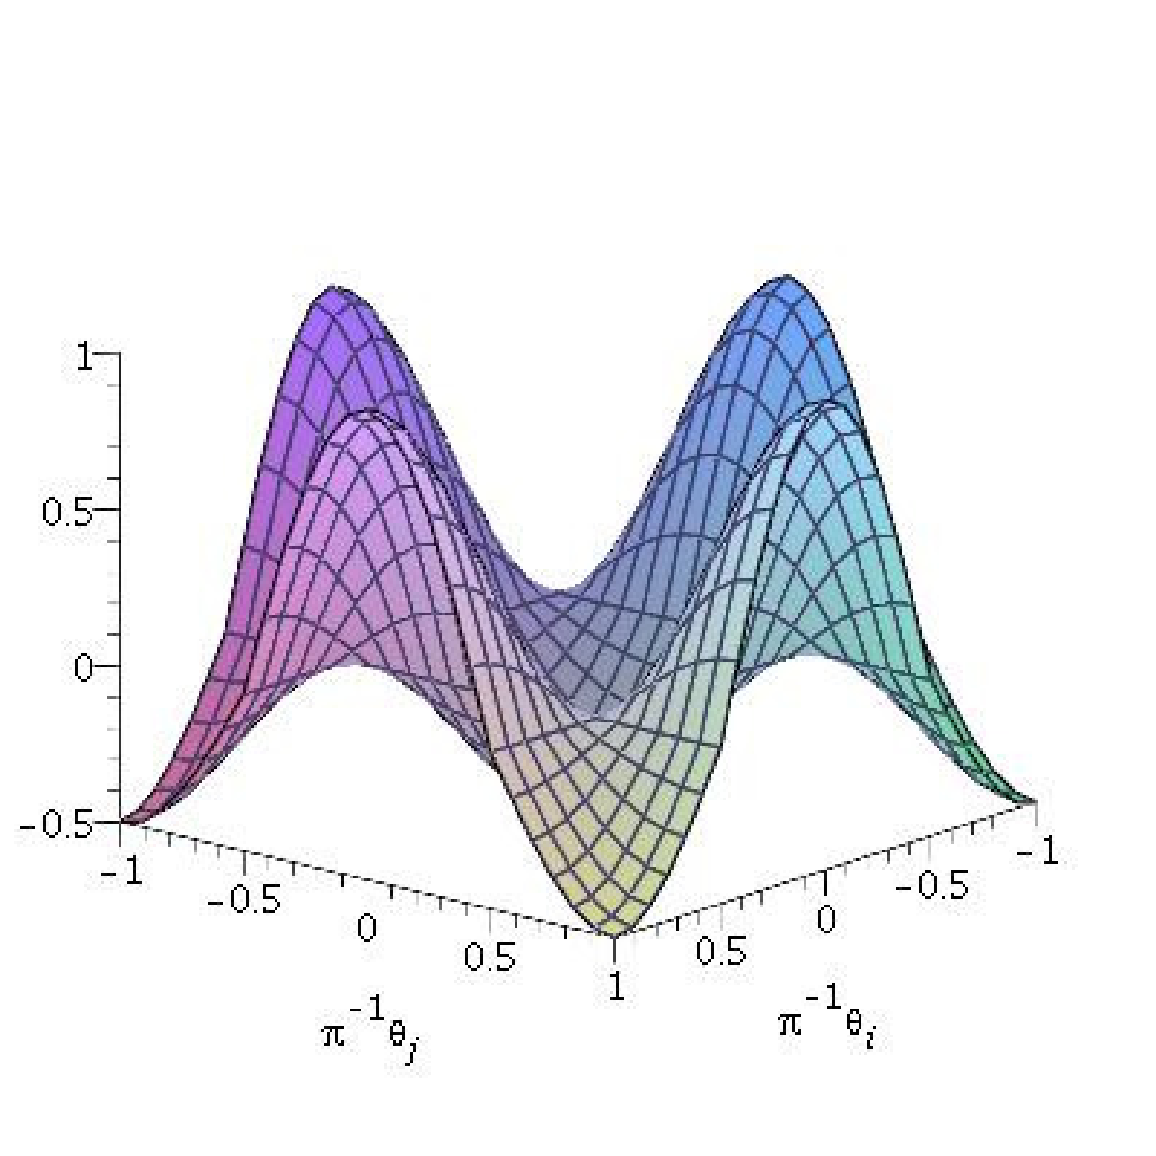
\includegraphics[width=\textwidth]{Figures/Vd5}
    \caption{$\delta = 0.5$}
\end{subfigure}    
%
\begin{subfigure}{0.31\textwidth }
    \centering
    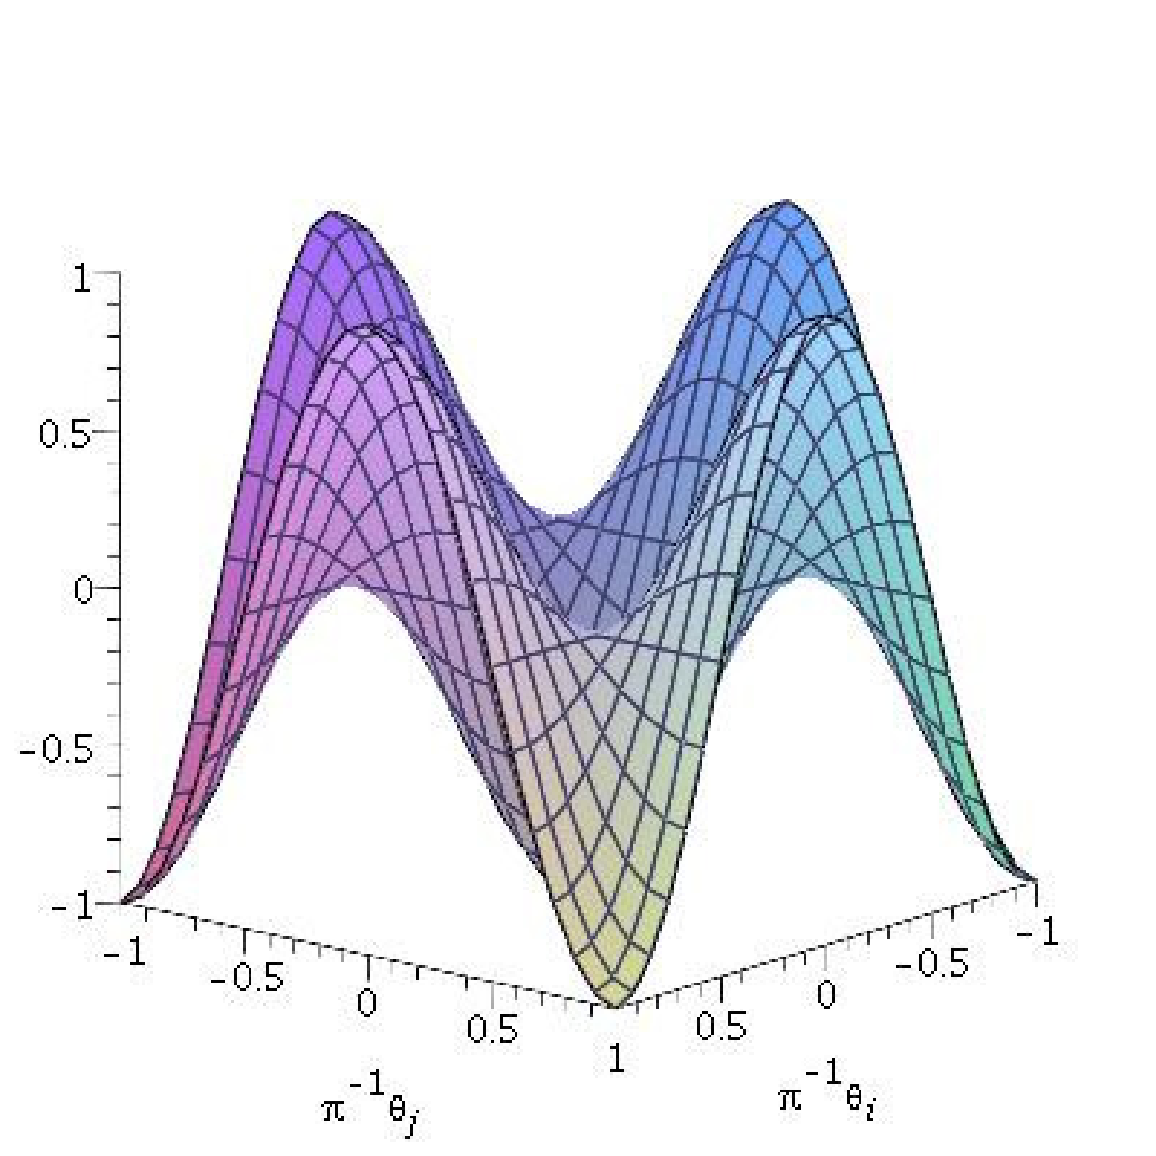
\includegraphics[width=\textwidth]{Figures/Vd10}
    \caption{$\delta = 1.0$}
\end{subfigure}
%
\label{fig:Vd}
\end{figure*}

Para entendermos a dinâmica da sociedade acompanharemos o histogramas ($q_h$),
médias ($m$) e variância ($v$) das opiniões dos agentes em relação ao
\textit{Zeitgeist} ($h_i = \bm{\omega}_i\cdot\mc Z$), que são definidos
respectivamente por
\begin{align}
q_h &= \frac{1}{K}\sum_{i=1}^K I\left( h_{i} = h \right), 
        \qquad h \in \left[-1, 1\right],\label{eq:overI1} \\
m &= \frac{1}{K}\sum_{i} h_{i}, \label{eq:M}\\
v &= \frac{1}{K-1}\sum_{i} \left(m - h_{i}\right)^2, \label{eq:V}\\
\end{align}
onde $ I \left( x \right) $ é função indicação , que assume o valor unitário
caso a asserção $ x$ seja verdadeira, e zero caso contrário. 

\begin{marginfigure}
\center
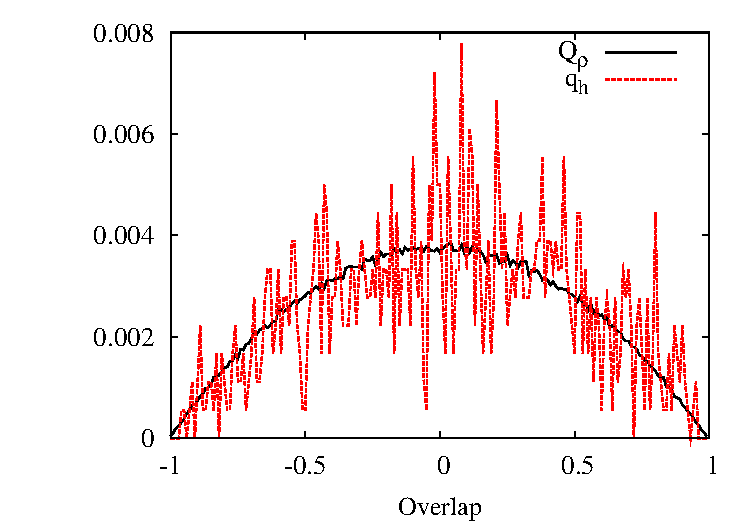
\includegraphics[width = \textwidth]{Figures/Ovelap_Vetores_Uniforme_Dim5_N900}
\caption{
    Figura com as distribuições dos sobreposições entre agentes $(Q_\rho)$
    e do sobreposição entre os agentes e o assunto discutido $q_h$ para
    $K = 900$ agentes com seus vetores sinápticos sorteados uniformemente
    sobre superfície de uma hiperesfera de $N=5$ dimensões. Vemos que a
    distribuição $Q_\rho$ apresenta menor flutuação que a distribuição
    $(q_h)$ pois é calculada levando-se em conta a combinação sobre todas
    as duplas de agentes.
}
\label{fig:J_uniform}
\end{marginfigure} 

Outra grandeza que pode ser usada para a análise do sistema é a
\textbf{similaridade} entre as opiniões dos agentes, que definiremos como o
produto escalar entre os vetores sinápticos entre dois agentes \footnote{Note
que a variável $\rho$ nesse contexto não tem nenhuma relação com o
parâmetro de aprendizado a função de modulação do aprendizado do agente
Bayesiano}$ \rho_{ij} = \bm{\omega}_i.\bm{\omega}_j$. Acompanhamos
o histograma ($Q_\rho$), média ($M$) e variância ($V$) dessa variável
considerando todas as duplas de agentes, independentemente se eles são ou
não vizinhos .
\begin{align}
    Q_\rho &= \frac{1}{D}\sum_{i<j}I\left( \rho_{ij} = \rho \right),
        \qquad \rho \in \left[-1, 1\right] \label{eq:overA1} \\
    M &= \frac{1}{D}\sum_{i<j} \rho_{ij}; \label{eq:M}\\ 
    V &= \frac{1}{D-1}\sum_{i<j}\left( M - \rho_{ij} \right)^2; \label{eq:V}
\end{align}
Onde $D = K\left(K-1\right)/2$ é o número total de duplas de agentes
na sociedade. A vantagem de calcularmos essas grandezas é que, levando em
consideração todas as duplas de agentes, obtemos uma flutuação menor quando
comparadas com as medidas similares das opinião dos agentes. Isso possibilita
uma melhor análise do perfil de opiniões dos agentes na sociedade sem que
seja necessário tirar médias temporais ou sobre diferentes experimentos de
monte carlo. Isso pode ser verificado atravéz da figura \ref{fig:J_uniform},
onde mostramos os histogramas da similaridade e opiniões dos agentes quando
os vetores sinápticos são distribuídos uniformemente sobre uma hiperesfera
de 5 dimensões.

\newpage
\section{Dependência com os parâmetros do modelo e diagramas de Fase} %#{{{2
\label{sec:deppar}

No modelo existem alguns parâmetros livres, os dois mais óbvios são
a pressão de pares $\alpha$ e a tendência corroborativa do agente
$\delta$. Outros parâmetros livres são os parâmetros usados para definir
o grafo  $\mc G$ de suporte da sociedade. Entre eles, o número médio de
vizinhos e o número total de agentes são os mais importantes.

Primeiramente vamos avaliar a influência dos parâmetros $\alpha$ e $\delta$
no estado de equilíbrio, olhando para os histogramas da similaridade dos
agentes mostrados na figura \ref{fig:hist1}. Na figura \ref{fig:hist1}(a)
fixamos o parâmetro de pressão $\alpha=0.6$ e calculamos o histograma
$Q_\rho$ para vários valores da tendência corroborativa dos agentes, sendo
que quanto mais vermelho menor o valor de $\delta$. Com isso, podemos ver
claramente, que quanto maior é a tendência corroborativa dos agentes mais
os histogramas se alinham para valores com uma maior similaridade entre os
agentes. Um efeito semelhante pode ser visto na figura \ref{fig:hist1}(b),
onde fixamos o valor da tendência corroborativa dos agentes $\delta = 0.2$
e calculamos os histogramas para diversos valores da pressão entre pares
$\alpha$. Vemos que quanto maior o valor de $\alpha$ mais similares são
os agentes.

\begin{figure*}
    \centering
    \begin{subfigure}[]{0.45\textwidth}
        \centering
        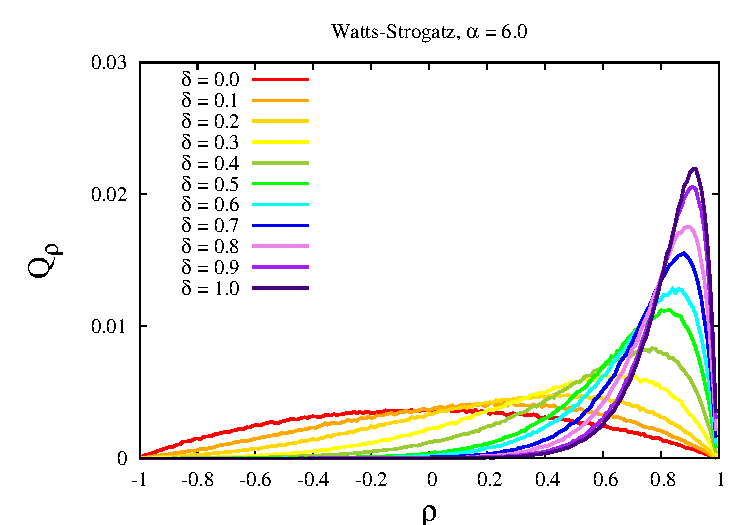
\includegraphics[width =\textwidth]{Figures/HistoDeltaBeta6}
        \caption{$\alpha = 0.6$}
        \label{fig:Histo-vd}
    \end{subfigure}
    \begin{subfigure}[]{0.45\textwidth}
        \centering
        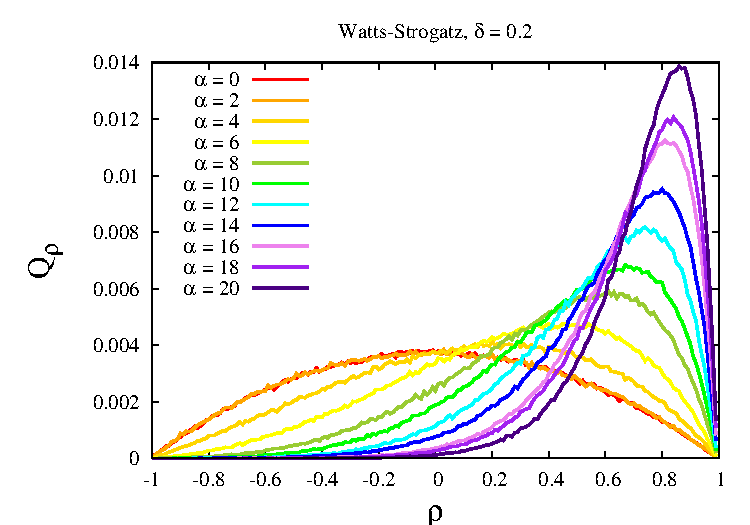
\includegraphics[width =\textwidth]{Figures/HistoBetaDelta02}
        \caption{$\delta = 0.2$}
        \label{fig:Histo-va}
    \end{subfigure}
    \newline
    \caption{Histogramas das similaridades entres os agentes $Q_\rho$.}
    \label{fig:hist1}
\end{figure*}

É importante notar na figura \ref{fig:hist1} que para alguns valores
pequenos dos parâmetros $\alpha$ e $\delta$ o histograma $Q_\rho$ é
o mesmo de uma sociedade totalmente desordenada que foi apresentado na
figura \ref{fig:J_uniform}. Esse fenômeno pode ser observado com mais
clareza nas figuras \ref{fig:ov}(a) e \ref{fig:ov}(c) \footnote{A escala
de cor da figura \ref{fig:ov} é a mesma que da figura \ref{fig:hist1}(a)}
onde mostramos as médias das opiniões e das similaridades dos agentes em
função da pressão de pares $\alpha$, para vários valores de $\delta$. Vemos
claramente que existe uma região onde $m=0$ e $M=0$, sendo que para um valor
de $\alpha_c(\delta)$ essas quantidades ficam maiores que zero. No caso da
média ( $m$ ) das opiniões dos agentes, essa mudança é abrupta o que
caracteriza uma transição de fase de segunda ordem. Isso também pode ser
verificado pois o gráfico \ref{fig:ov}(d) onde apresentamos o gráficos
da variância das opiniões dos agentes, que sofrem variações abruptas
em suas derivadas na mesma região de parâmetro onde a opinião média se
torna positiva. O fenômeno da transição de fase nesse sistema também
foi estudado nas referências \citep{Caticha2011a,Susemihl2010}.

\begin{figure*}
    \centering
    \begin{subfigure}[]{0.45\textwidth}
        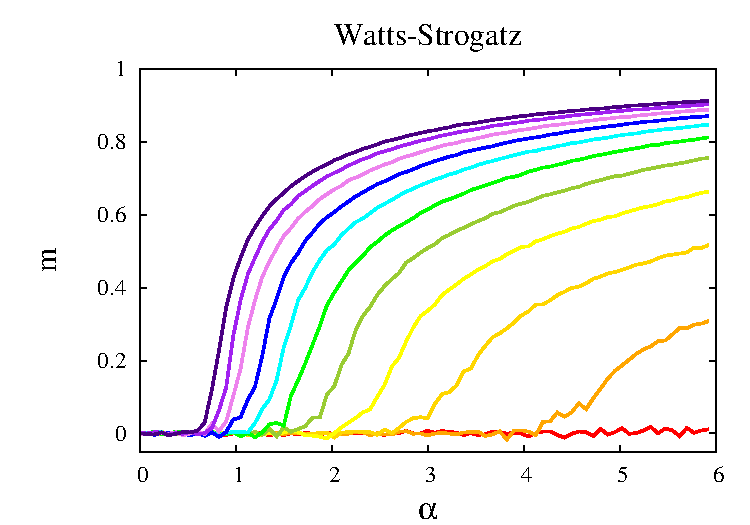
\includegraphics[width = \textwidth]{Figures/DeltaXBeta_Mag}
        \caption{$m\times\alpha$}
        \label{fig:fm}
    \end{subfigure}
    \begin{subfigure}[]{0.45\textwidth}
        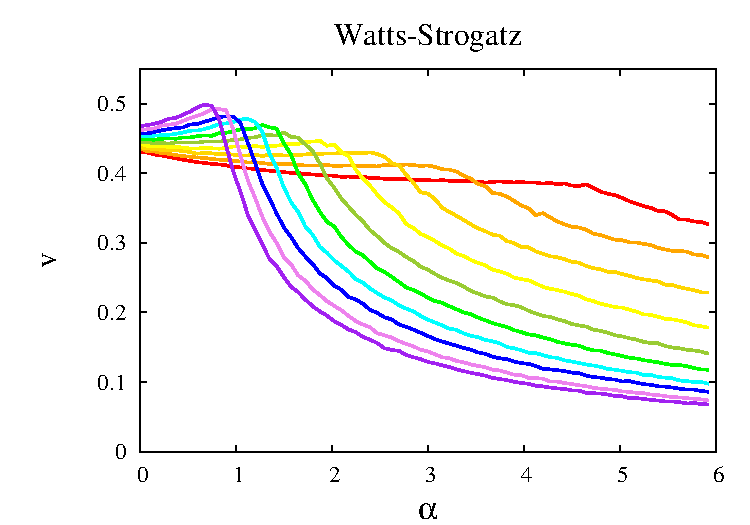
\includegraphics[width = \textwidth]{Figures/DeltaXBeta_Var}
        \label{fig:fv}
        \caption{$v\times\alpha$}
    \end{subfigure}
    \begin{subfigure}[]{0.45\textwidth}
        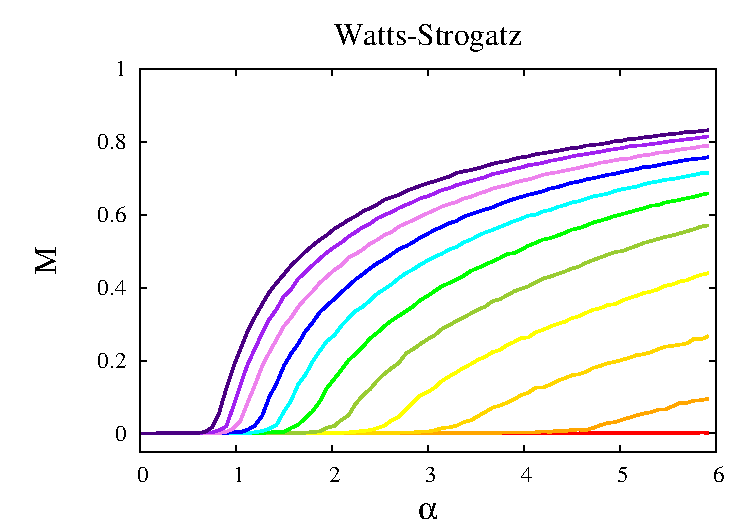
\includegraphics[width = \textwidth]{Figures/DeltaXBeta_MMag}
        \label{fig:fM}
        \caption{$M\times\alpha$}
    \end{subfigure}
    \begin{subfigure}[]{0.45\textwidth}
        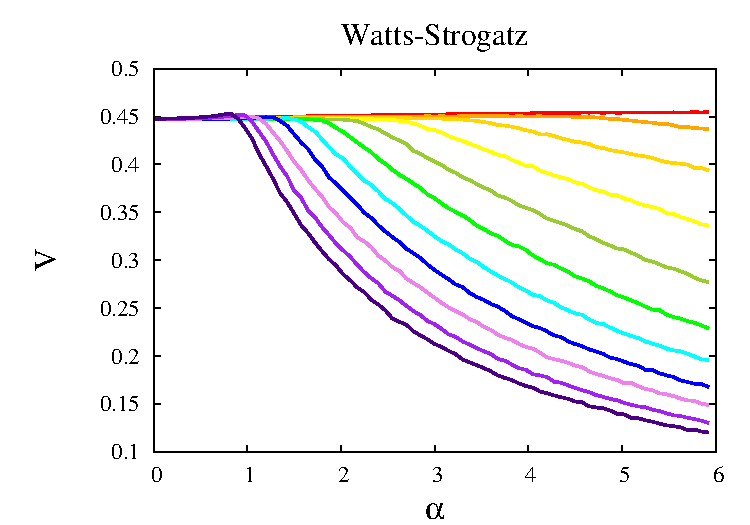
\includegraphics[width = \textwidth]{Figures/DeltaXBeta_VVar}
        \label{fig:fV}
        \caption{$V\times\alpha$}
    \end{subfigure}
    \newline
    \caption{ 
        Gráficos com os valores das médias $m$ , $M$ e variâncias  $v$, $V$
        de equilíbrio em função do parâmetro $\alpha$ para vários valores
        de $\delta$. simulações, numa rede Watts-Strogatz e $K=900$ agentes
        com número médio de vizinhos $n=4.0$, média de uma amostragem 20
        experimentos.
    }
    \label{fig:ov}
\end{figure*}

Nas figuras \ref{fig:DiagFase} e \ref{fig:DiagFaseDif}, apresentamos
linhas de transição de fase que foram calculadas marcando os pontos nos quais a
similaridade média dos agentes supera um pequeno valor de limiar ($M>\epsilon$).

\begin{figure}
\centering
\caption{ 
    Diagramas de fase para sociedades de tamanhos diferentes. A curva separa
    uma região de parâmetros que viabiliza o consenso da sociedade, sendo
    que a parte de baixo não viabiliza. Consideramos que existia consenso
    se o sobreposição médio entre as opiniões dos agentes fossem maior que um
    limiar ($M > \epsilon $).  Calculamos esse gráfico com os agentes em
    uma rede do tipo Barabasi-Albert com $K=900$ e com número médio de
    vizinhos $n=4$. Para $K =900$ agentes os pontos e suas barras de erro
    foram obtidos através de 10 simulações independentes, para $K=400$ usamos
    15 simulações e para $K=100$ usamos 30 simulações. 
    }
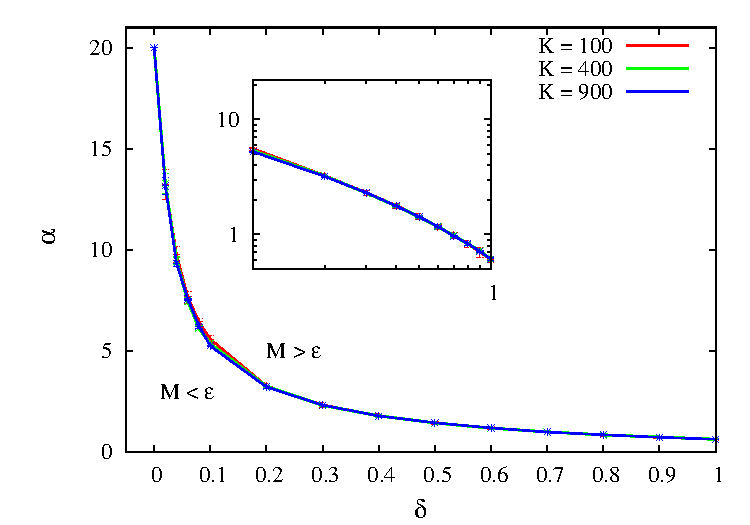
\includegraphics[width=0.9\textwidth]{Figures/Diag_AgentAgent_Barabasi_Dif_NUM_Nviz4}
\label{fig:DiagFase}
\end{figure}

Na figura \ref{fig:DiagFase} calculamos o diagramas de fase para uma sociedade
distribuída numa rede Watts-Strogatz com diferentes tamanhos. Podemos
observar que a linha da transição de fase não depende do numero total
de agentes. Já na figura \ref{fig:DiagFaseDif}(a) calculamos o diagrama de
fase para sociedades com 900 agentes distribuídos sobre diferentes grafos
de suporte. Também observa-se através desse gráfico que existe pouca
dependência da região de transição de fase com a estrutura topológica
da sociedade. 

\begin{figure}
    \centering
    \begin{subfigure}[]{.8\textwidth}
        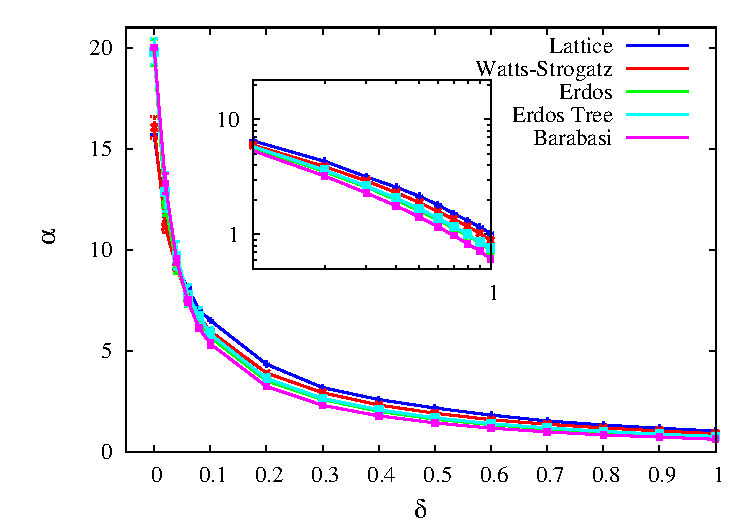
\includegraphics[width=\textwidth]{Figures/Diag_AgentAgent_N400_Nviz4}
        \caption{}
        \label{fig:FaseRede}
    \end{subfigure}
    \begin{subfigure}[]{.8\textwidth}
        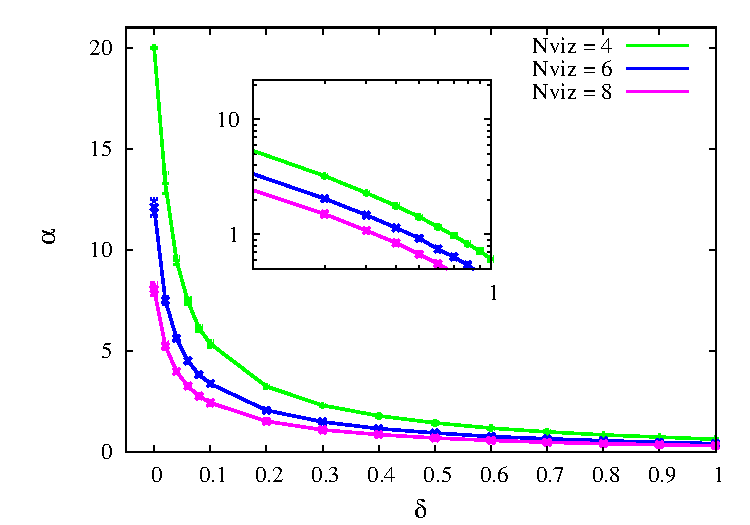
\includegraphics[width=\textwidth]{Figures/Diag_AgentAgent_Barabasi_N400_Dif_Nviz}
        \label{fig:FaseVis}
        \caption{}
    \end{subfigure}
    \caption{
        Diagramas de fase calculados para diferentes redes e com diferentes
        números médios de vizinhos:  As figuras acima foram calculadas com
        $K = 900$ agentes e os pontos e suas barras de erro foram feitos
        a partir de 20 simulações.  Na figura (a) os diagramas de fase
        foram calculado para diferentes grafos. Percebemos através desse
        gráfico que a estrutura da sociedade tem pouca interferência
        sobre o comportamento dessa transição fase. Já na figura (b),
        calculamos o diagrama de fase, com $K=900$ agentes dispostos sobre
        uma rede Barabasi-Albert, para diferentes números médio de vizinhos
        por sítio. Percebemos, por esse gráfico, que quanto maior o número
        médio de vizinhos, menor é o parâmetro $\alpha$ para o qual ocorre
        a transição de fase. Isso ocorre devido ao fato de que quanto mais
        vizinhos um agente tem, maior é a variação da energia causada
        por uma mudança no seu vetor de opinião.
    } 
    \label{fig:DiagFaseDif}
\end{figure}

Por fim, avaliamos através da figura \ref{fig:DiagFaseDif}(b) a
dependência da transição de fase com o número médio de vizinhos numa rede
do tipo Barabasi-Albert com 900 agentes. Como já é esperado a transição
de fase ocorre para valores mais baixos do parâmetro de pressão social
já que a energia de interação de uma agente com sua vizinhança cresce
como o número de vizinhos.

\newpage
\section{Consenso e Polarização} %#{{{2

O parâmetro $\delta$ da função de modulação, apesar de representar uma
tendência natural do agente entrar em conformidade com seus vizinho, dá
origem a uma importante característica desse modelo de opinião, que é a
sua capacidade de criar estados polarizados. Essa característica foi pela
primeira vez evidenciada na referência \cited{Vicente2009} para o caso em
que o grafo de suporte da sociedade é um anel. Neste trabalho, a dinâmica
do aprendizado dos agentes é feita através do algoritmo de aprendizado
\eqref{eq:Japrende} mas sem incorporar nenhum ruído ao sistema. No nosso
cenário de aprendizado, isso equivale a uma dinâmica de Monte Carlo com
uma pressão social infinita ( $\alpha \rightarrow \infty $). É importante
salientar que os resultados apresentados nesta secção são obtidos partir
de simulações onde a condição inicial dos vetores sinápticos de cada agente
é sorteada uniformemente em uma hiperesfera de 5 dimensões.

\begin{figure*} 
  \centering
  \begin{subfigure}[]{0.5\textwidth}
  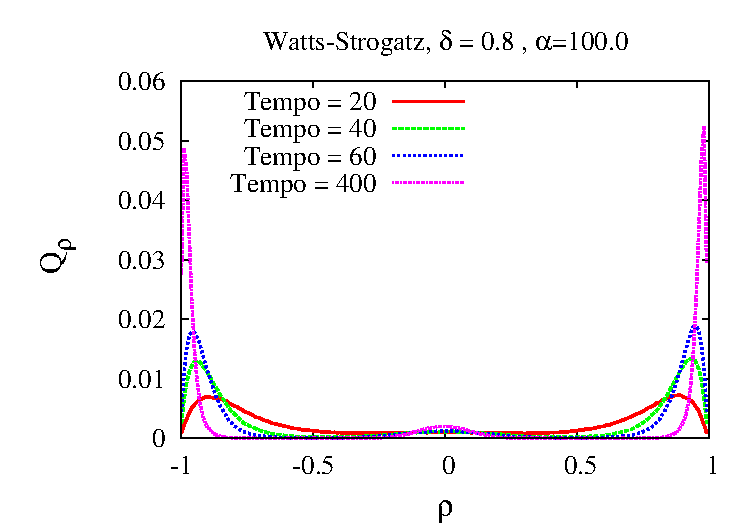
\includegraphics[width = \textwidth]{Figures/Histograma_Watts_Strogatz_Polariza}
  \caption{Distribuição $Q_\rho$ calculada para vários tempos}
  %\label{fig:Histo_Pol1}
  \end{subfigure}
  \begin{subfigure}[]{0.45\textwidth}
  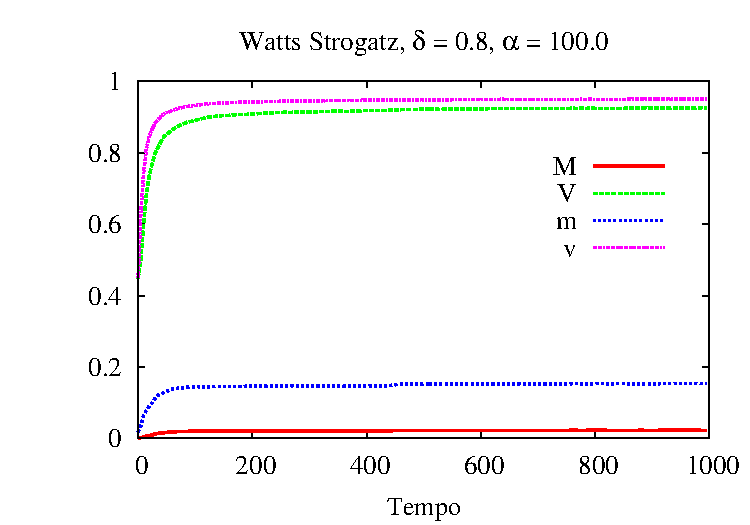
\includegraphics[width = \textwidth]{Figures/MagTempo_Polariza}
  \newline
  \caption{Evolução temporal das médias e variâncias dos sobreposições}
  %\label{fig:Mag_Pol}
  \end{subfigure}
  \newline
  \caption{
      Figuras com a evolução temporal do processo de polarização da
  sociedade. Na figura (a) a sociedade se divide em duas facções
  uma distribuída em torno do \textit{Zeitgeist} e outra na direção
  contraria. Já na figura (b) é apresentado a evolução
  temporal da média e variância do sobreposições. Os gráficos foram
  obtidos através de um experimento de Monte Carlo com $\alpha = 100$
  e $\delta = 0.8$ para $K = 1089$ agentes que estão distribuídos sobre
  uma rede do tipo Watts-Strogatz, com número médio de vizinhos $n=4$
  e probabilidade de redistribuição de vértices $p=0.1$.
  }
  \label{fig:Pol}
\end{figure*}

Na figura \ref{fig:Pol} mostramos uma rodada de Monte Carlo na qual a
dinâmica do processo leva a um estado polarizado. Observa-se através
dos histogramas $Q_\rho$ para diferentes tempos de simulação que são
apresentados na figura \ref{fig:Pol}(a), que a sociedade se divide em duas
facções, uma que se distribui na direção do \textit{Zeitgeist} e outra na
direção contaria. Observa-se também,  através da figura \ref{fig:Pol}(b),
onde é apresentado as médias e variâncias das opiniões e similaridades dos
agentes, que a polarização da sociedade sobrevive para tempos longos de
simulação. Essa simulação foi feita com alta pressão entre pares, $\alpha
= 100$, e com agentes com grande tendência de entrar em conformidade,
$\delta = 0.8$. Usamos $K = 1039$ agentes distribuídos sobre uma rede do
tipo \textit{Watts-Strogatz} (também conhecida como rede de mundo pequeno)
com um número de vizinhos por sítio $n = 4$ , e com um grau de rearranjo
$p = 0.1$. 

Podemos observar pela figura \ref{fig:Pol}(b) que, como a pressão social
é muito grande, o sistema rapidamente atinge um estado de equilíbrio
metaestável. Além disso, como $m\approx0.15$ vemos que o tamanho dos
domínios de agentes que estão na direção do \textit{Zeitgeist} é um
pouco maior que o domínio na direção contraria.

\begin{figure*}
    \centering
    \begin{subfigure}[]{0.5\textwidth}
        \centering
        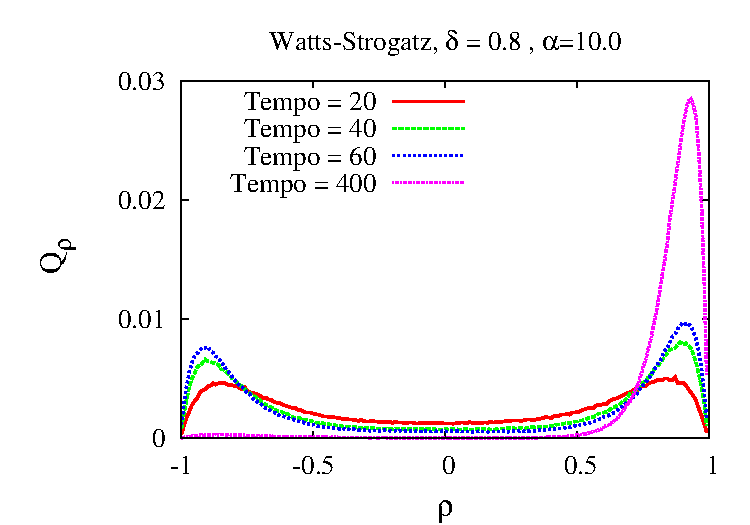
\includegraphics[width = \textwidth]{Figures/Histograma_Watts_Strogatz_Consenso}
        \caption{}
       %\label{fig:Histo_Con}
    \end{subfigure}
    \begin{subfigure}[]{0.45\textwidth}
        \centering
        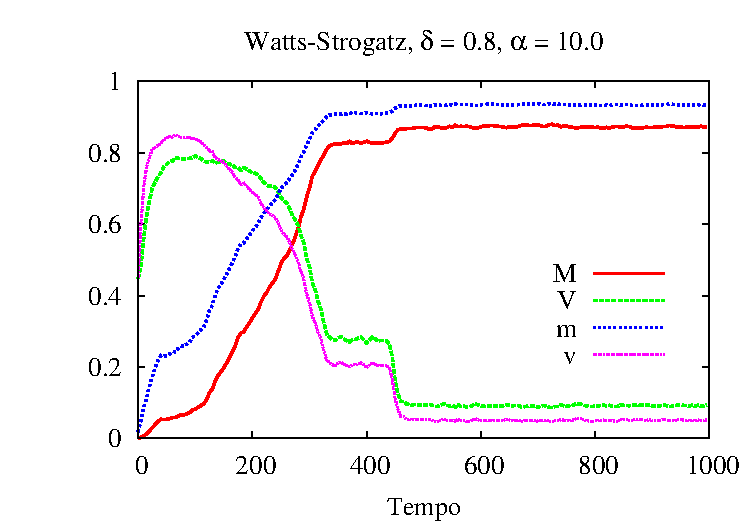
\includegraphics[width = \textwidth]{Figures/MagTempo_Consenso}
        \caption{}
       %\label{fig:Mag_Con}
    \end{subfigure}
    \newline
    \caption{
        Figuras com a evolução temporal da sociedade em uma dinâmica que
        leva a um estado consenso.  São apresentados (a) as distribuições
        $Q_\rho$ em diversos tempos. Inicialmente a dinâmica leva a estados
        polarizados.  Com o passar do tempo uma das facções é destruída
        e o estado de equilíbrio é um estado de consenso. Na figura (b)
        é apresentado a evolução temporal das médias e variâncias das
        opiniões e similaridade dos agentes.  A simulação é feita sob
        as mesmas condição das apresentadas na figura \ref{fig:Pol}, exceto
        o parâmetro de pressão social que é $\alpha=10$.
    } 
    \label{fig:Con}
\end{figure*}


No entanto, para pressões sociais menores as opiniões dos agentes são mais
suscetíveis a flutuações. Isso faz com que a dinâmica da sociedade deixe
de ser capaz de sustentar estados polarizados. Esse comportamento pode ser
observado na figura \ref{fig:Con}, que é obtida sobre as mesmas condições
que a figura \ref{fig:Pol}, exceto pelo parâmetro do inverso da temperatura,
que será $\alpha = 10$. Observa-se pela figura que inicialmente existe uma
tendência de se criarem facções, no entanto, subitamente o sistema
alcança o estado de equilíbrio que é o concesso.

\begin{figure*}
\centering
\begin{subfigure}[]{0.45\textwidth}
    \centering
    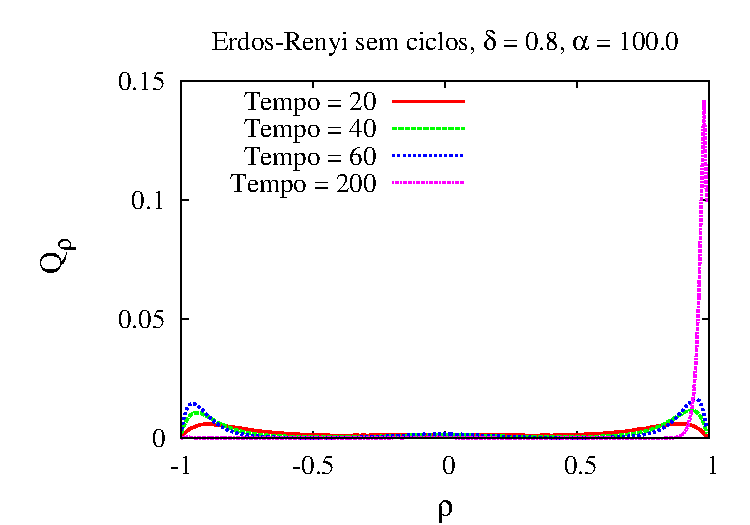
\includegraphics[width = \textwidth]{Figures/Histograma_Arvore}
    \caption{}
    %\label{fig:Histo_Arvore}
\end{subfigure}
\begin{subfigure}[]{0.45\textwidth}
   \centering 
    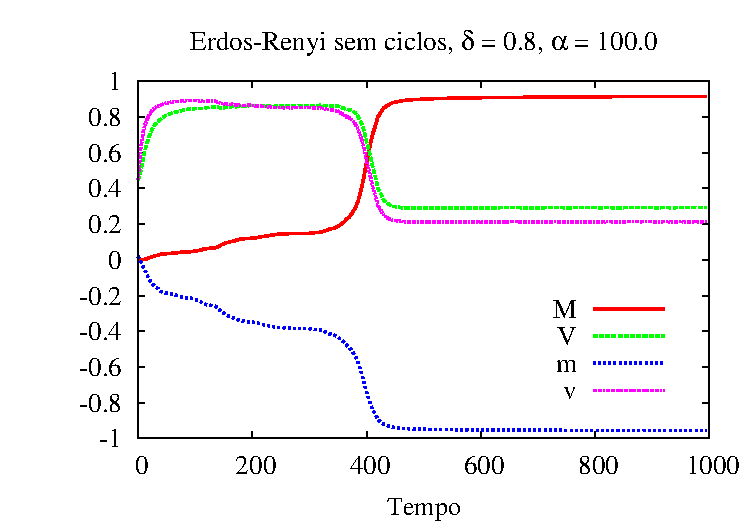
\includegraphics[width = \textwidth]{Figures/MagTempo_Arvore}
   \caption{}
    %\label{fig:Mag_Arvore}
\end{subfigure}
\newline
\caption{
    Figuras com a evolução temporal da sociedade em uma dinâmica que leva
    a um estado consenso. Os gráficos acima foram obtidos a partir de uma uma
    rodada de simulação de Monte Carlo com $\alpha = 100$ e $\delta = 0.8$ para
    $K = 1089$ agentes que estão distribuídos sobre uma arvore aleatória.
}
\label{fig:Arvore}
\end{figure*}

Os mecanismos que levam esse sistema a estados polarizados precisam ainda
ser melhor compreendidos. Sabemos que existe uma forte dependência deste
fenômeno com a estrutura do grafo de suporte da sociedade e com condição
inicial da distribuição de opiniões dos agentes sobre esse grafo. Na
figura \ref{fig:Arvore} apresentamos o resultado de uma rodada de Monte
Carlo feita sob as mesmas condições da figura \ref{fig:Pol}, com exceção
do grafo de suporte da sociedade. Nessa simulação foi usado uma árvore
aleatória ou grafo do tipo Erdös-Rényi sem ciclos. Vemos que mesmo
com uma pressão social extremamente alta ($\alpha = 100$), a estrutura da
sociedade não permite a manutenção de estados polarizados, pois em um
curto intervalo de tempo a sociedade passa de um estado polarizado para um
estado de consenso.  É interessante observar que o estado de equilíbrio
atingindo na dinâmica é um estado de consenso em que as opiniões dos
agentes estão na direção contrária do assunto discutido ($m \approx -1$)
. Esse tipo de comportamento é esperado devido ao fato da Hamiltoniana do
sistema \ref{eq:H1} ser simétrica sobre a transformação $\bm{\omega}_i
\rightarrow -\bm{\omega}_i$ para todo $i$.


\newpage
\section{Diferentes Estratégias Cognitivas} %#{{{2
\label{sec:dd}

Numa sociedade real, pessoas com diferentes estratégias cognitivas convivem
entre si e suas interações alteram suas percepções sobre os mais diversos
assuntos. Podemos tentar implementar esse fato em nosso modelagem da maneira
mais direta possível; impondo que cada agente, com vetor de opinião
$\bm{\omega}_i$, tenha uma estratégia cognitiva própria, representada por
$\delta_i$ na sua função de aprendizado.  Fazendo isso, o potencial de
interação do agente $i$ com um de seus vizinhos $j$ será dado por.
\begin{equation}
V_{\delta_i}\left(h_i,h_j\right) = -\frac{1 + \delta_i}{2}h_ih_j 
        + \frac{1 + \delta_i}{2}\left|h_ih_j\right| 
\end{equation}

Na dinâmica, quando esse agente é escolhido ao acaso para interagir
com seu vizinho, ele tentará aprender a opinião dele usando a equação
\ref{eq:Japrende}. Como foi feito anteriormente, o agente aceita a mudança
na sua opinião se isso diminuir a energia interação com sua vizinhança,
caso contrário ele aceita essa mudança com uma probabilidade
\begin{equation}
p_i = \exp\left(-\alpha\sum_{j
    \in\mathcal{V}_i} \left[V_{\delta_i}^{new}\left(h_i,h_j\right)
    -  V_{\delta_i}^{old}\left(h_i,h_j\right) \right]\right), 
\end{equation}
onde $\mathcal{V}_i$ é a vizinhança do agente $i$. 

\begin{figure}
\centering
    \begin{subfigure}[]{.9\textwidth}
        \centering
        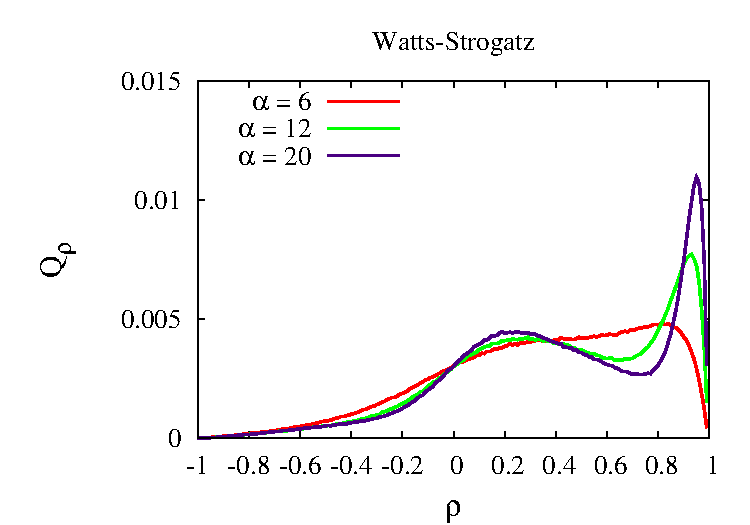
\includegraphics[width=\textwidth]{Figures/ComparaHistoD01Beta}
        \caption{Histograma sociedade completa}
        %\label{fig:}
    \end{subfigure}
    \begin{subfigure}[]{.9\textwidth}
        \centering
        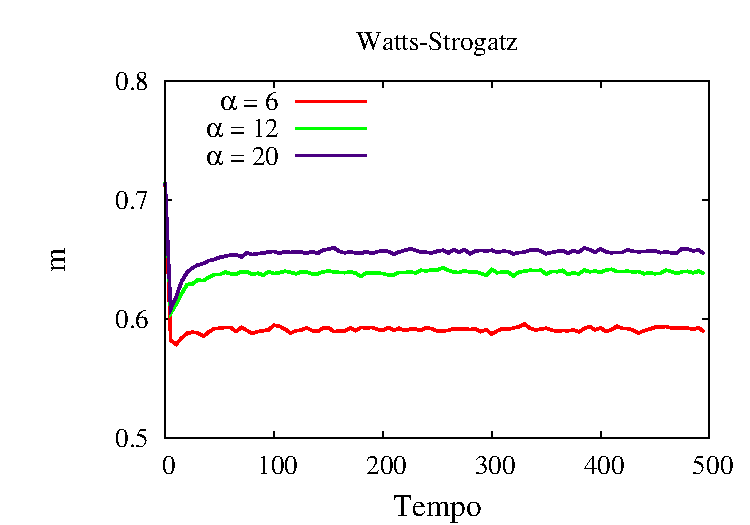
\includegraphics[width=\textwidth]{Figures/MagCompleto1Beta}
        \caption{Evolução temporal sociedade completa}
        %\label{fig:}
    \end{subfigure}
\label{fig:DDCompleto} \caption{Figura com os histogramas e médias dos
sobreposições entre agentes com a mesma estratégia cognitiva $\delta$
numa sociedade na qual metades dos agentes têm $\delta = 0$ e outra metade
tem $\delta =1$. Na figura (a) apresentamos os histogramas da similaridade
entre todos os agentes ($Q_\rho$) para diferentes valores de pressão
de pares $\alpha$, enquanto em (b) apresentamos evolução temporal das
médias das opiniões de todos os agentes ($m$). Essas figuras foram feitas
com $K=2500$ agentes com número médio de vizinhos $n=4$ numa rede do
tipo $Watts-Strogatz$. Os gráficos dos histogramas foram feitos usando uma
rodada de simulação enquanto os gráficos da média dos sobreposições
foram construídos com 10 simulações. }
\end{figure}

Por simplicidade, analisamos o caso extremo onde metade dos agentes têm a
tendência a concordância máxima ($\delta = 1$) e a outra metade mínima
($\delta = 0$). A estratégia cognitiva do agente é sorteada independentemente
da sua vizinhança com probabilidade 1/2.  Como a interação entre os
agentes não é simétrica não podemos definir uma Hamiltoniana para o
sistema, no entanto, isso não impede que a dinâmica do modelo leve a
estados estacionários como observa-se nas figuras \ref{fig:DDCompleto}
e \ref{fig:DDSeparado}.

Na figura \ref{fig:DDCompleto}(b) apresentamos a média das opiniões dos
agentes sobre \text{Zeitgeist} ($m$) para diferentes valores do parâmetro
$\alpha$. Primeiramente, observa-se nessa figura que existe uma tendência
de diminuição do consenso na sociedade, no entanto, esse comportamento é
rapidamente revertido e a sociedade entra em equilíbrio num estado macroscópico
de consenso que cresce em função do parâmetro $\alpha$. Nesse cenário,
vemos um comportamento curioso quando analisamos o histograma de $Q_\rho$
para diferentes valores do parâmetro $\alpha$, como é apresentado na figura
\ref{fig:DDCompleto}(a). Observa-se que à medida que $\alpha$ cresce surgem
duas facções na sociedade, uma com bastante consenso e outra facção 
com bastante dispersão entre seu agentes.

\begin{figure*}
    \centering
    \begin{subfigure}[]{0.45\textwidth}
        \centering
        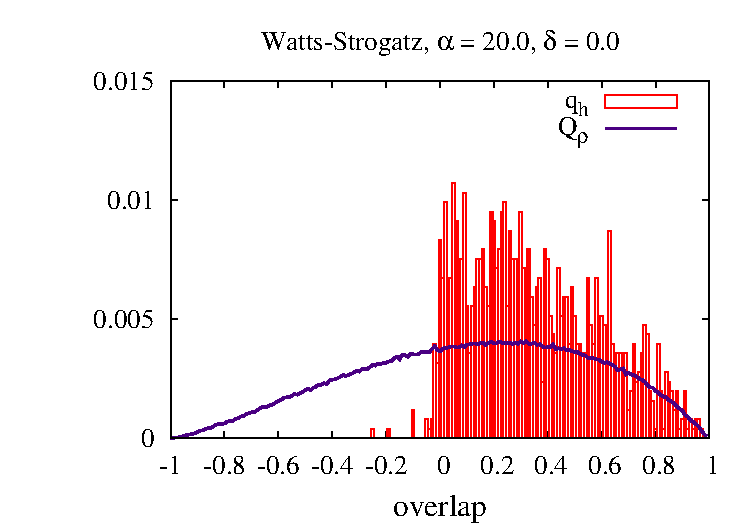
\includegraphics[width=\textwidth]{Figures/HistoDeltaD0Beta20}
        \caption{Histogramas $\delta = 0$}
        %\label{fig:}
    \end{subfigure}
    \begin{subfigure}[]{0.45\textwidth}
        \centering
        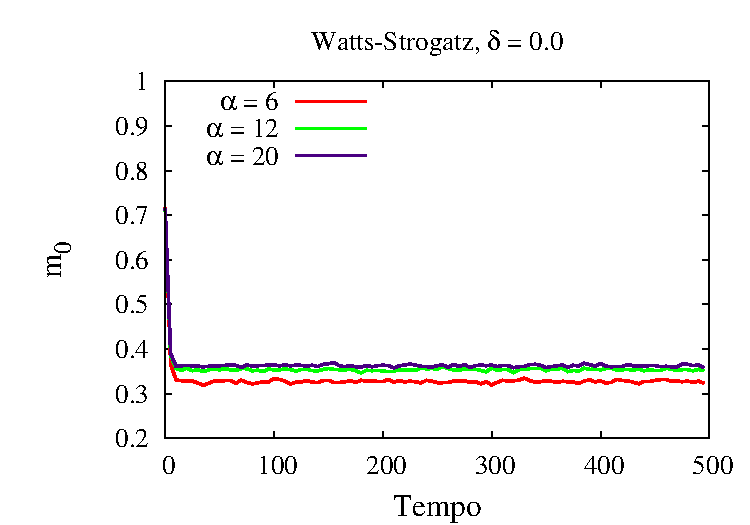
\includegraphics[width=\textwidth]{Figures/MagD0Beta}
        \caption{Evolução $\delta = 0$}
        %\label{fig:}
    \end{subfigure}
    \begin{subfigure}[]{0.45\textwidth}
        \centering
        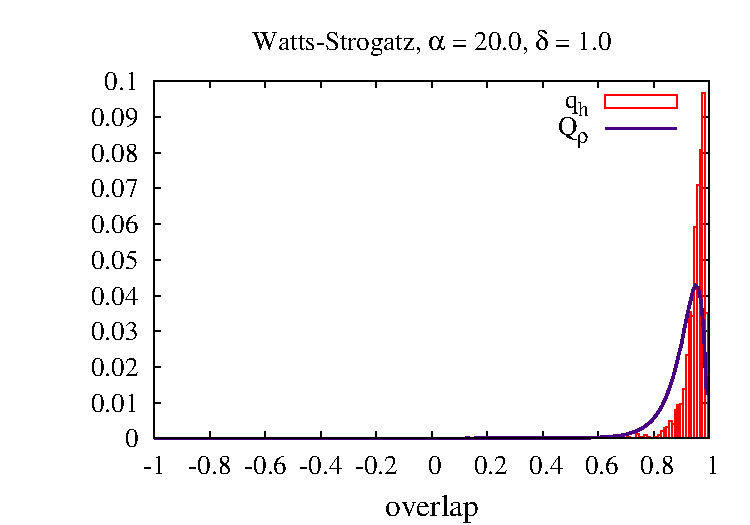
\includegraphics[width=\textwidth]{Figures/HistoDeltaD1Beta20}
        \caption{Histogramas $\delta = 1$}
        %\label{fig:}
    \end{subfigure}
    \begin{subfigure}[]{0.45\textwidth}
        \centering
        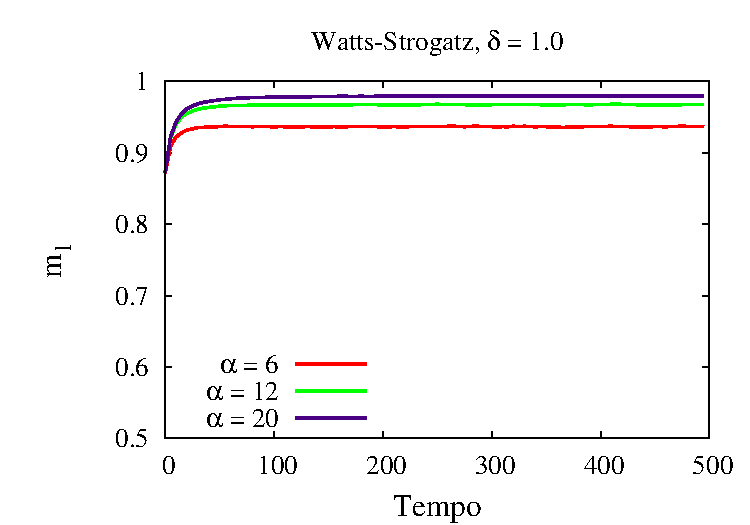
\includegraphics[width=\textwidth]{Figures/MagD1Beta}
        \caption{Evolução $\delta = 1$}
        %\label{fig:}
    \end{subfigure}
    \newline
    \caption{
        sociedade com $K=2500$ agentes sobre um grafo do tipo Watts-Strogatz
        com número médio de vizinhos $n=4$. O histograma foi obtido usando uma
        rodada de simulação e o gráfico com a média dos sobreposições foi obtido
        através de 20 rodadas de simulação.
        }
    \label{fig:DDSeparado}
\end{figure*}

O efeito da interação entre agentes com estratégias cognitivas diferentes
pode ser melhor avaliado a partir da figura \ref{fig:DDCompleto} onde
apresentamos o histogramas $Q_\rho$ e $q_h$ e a média $m$ do sobreposição
para agentes que tem o mesmo tipo de estratégia cognitiva. Observa-se pelas
figuras \ref{fig:DDSeparado}(a) e \ref{fig:DDSeparado}(b) que os agentes com
$\delta = 0$, devido à interação com agentes  de $\delta = 1$ se alinham
entorno do \textit{Zeitgeist}, pois para valores de pressão social menores
que $\alpha = 16$ (ver figura \ref{fig:DiagFaseDif}(a))
 é esperado que o estado de equilíbrio de agentes com essa estratégia
 seja totalmente desorganizados, ou seja, $m=0$. Vemos pelas figuras
\ref{fig:DDSeparado}(c) e \ref{fig:DDSeparado}(d) que o efeito oposto o corre
para agentes com $\delta = 1$ porem numa escala bem menor já esses agentes
tem uma grande tendência a se alinharem ao redor do Zeitgeist. É importante
salientar que a forma geral dos histogramas de opinião para agentes como a
mesma estratégia cognitiva não sofre grandes modificações \footnote{Por
exemplo, os histogramas não se tornam bimodais, ou sofrem mudanças mais
drásticas}, no entanto, um estudo mais detalhado sobre o comportamento da
sociedade de agentes com diferentes estratégias ainda precisa ser feito.

\newpage
\section{Convencimento de Populações} %#{{{2

No modelo de opinião que tratamos até aqui, os agentes sempre discutiam
um assunto fixo, ao qual denominamos de \textit{Zeitgeist}. Dessa forma,
no estado de equilíbrio os agentes ficam distribuídos ao redor de uma
direção fixa no espaço das opiniões. Vemos então que  esse procedimento
não nos permite avaliar como se dá a evolução do Zeitgeist na sociedade.
Para tanto, iremos flexibilizar um pouco o modelo da seguinte maneira:
após um tempo de termalização onde a sociedade discute um assunto fixo,
o \textit{Zeitgeist} discutido a cada passo da interação é calculado a partir
das média dos vetores sinápticos dos  agentes, ou seja,
\[
 \mc Z(t) \propto \frac{1}{K}\sum_i \bm \omega_i(t) = \mean{\bm \omega_i(t)}.
\]

\begin{figure*}
    \centering
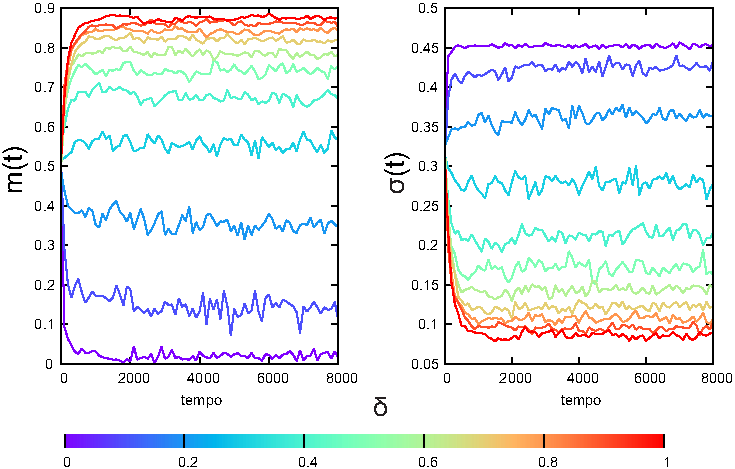
\includegraphics[width=0.9\textwidth]{Figures/evolveTermo}
\caption{
        Figura com a evolução temporal da média e variância entre o
    alinhamento do agentes e \textit{Zeitgeist} para vários valores de
    $delta$ e com a pressão social $\alpha = 8$, numa rede quadrada com
    400 agentes. Até o tempo = 1000, a evolução temporal é feita com
    o \textit{Zeitgeist} fixo, a partir desso ponto a evolução temporal
    é feita com o \textit{Zeitgeist} calculado a partir das médias das
    opiniões. Percebemos que a evolução dessas grandezas permanece
    praticamente inalterada com a nova dinâmica.
}
\label{fig:evolveTermo}
\end{figure*}

Com esse procedimento, esperamos que a direção do \textit{Zeitgeist} entre em
deriva. Para acompanharmos a dinâmica do modelo calculamos as médias e
variâncias das opiniões dos agentes sobre o \textit{Zeitgeist} instantâneo,

\begin{align}
m(t) &= \mean{\bm \omega_i(t)\cdot \mc Z(t)}, \nn 
\sigma(t) &= \frac{1}{K}\mean{\left(\bm \omega_i(t)\cdot \mc Z(t)\right)^2}
    - \mean{\bm \omega_i(t)\cdot \mc Z(t)}^2. \nn 
\end{align}

Essa modificação não muda de forma significativa a distribuição
de opiniões do estado de equilíbrio em relação ao assunto discutido,
como podemos ver na figura \ref{fig:evolveTermo} onde é mostrado a
evolução temporal da média e variância entre o alinhamento do agentes e
\textit{Zeitgeist} instantâneo. Até o tempo = 1000, a evolução temporal
é feita com o \textit{Zeitgeist} fixo, a partir desso ponto a evolução
temporal é feita com o \textit{Zeitgeist} calculado a partir das médias das
opiniões. Percebemos que a evolução dessas grandezas permanece praticamente
inalterada com a nova dinâmica.

\begin{figure*}
\centering
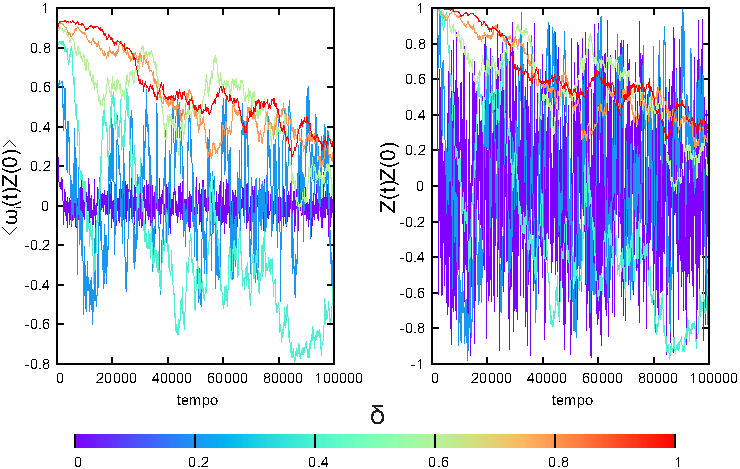
\includegraphics[width=0.9\textwidth]{Figures/evolveAngulosSemFixos}
\caption{Figura com movimento de deriva do \textit{Zeitgeist}. É mostrado a
média do alinhamento dos agentes com o \textit{Zeitgeist} inicial, e o produto
escalar entre o \textit{Zeitgeist} inicial e o instantâneo. Observa-se nessa
figura, que quanto menor o valor do parâmetro $\delta$ mais facilmente
os agentes perdem a memória do \textit{Zeitgeist} inicial. Figura
simulação feita com 400 agentes dispostos sobre uma rede quadrada.}
\label{fig:evolveAngulosSemFixos}
\end{figure*}

O movimento de deriva do \textit{Zeitgeist} pode ser analisado através
da figura \ref{fig:evolveAngulosSemFixos}, onde mostramos na esquerda
a média do alinhamento entre os agentes e o \textit{Zeitgeist} inicial
$\mean{\bm \omega_i(t)\cdot\mc Z(0)}$, e na direita o alinhamento entre
o \textit{Zeitgeist} instantâneo e o inicial $\mc Z(t)\cdot \mc Z(0)
$. Podemos constatar que, de fato, o \textit{Zeitgeist} apresenta um movimento
de deriva e, além disso, vemos que quanto menor o valor do parâmetro
$\delta$ mais facilmente os agentes perdem a memória do \textit{Zeitgeist}
inicial e mais acentuado são as flutuações das opiniões.

\begin{figure*}
\centering
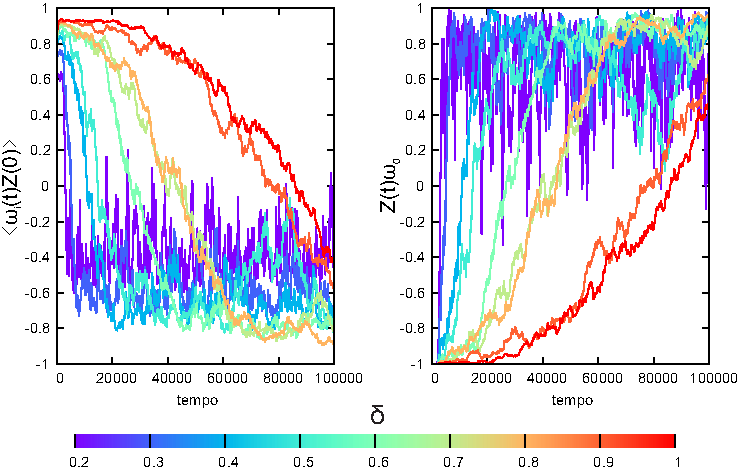
\includegraphics[width=0.9\textwidth]{Figures/evolveAngulosInit}
\caption{Figura com a média dos alinhamentos entre as opiniões dos agentes
e o \textit{Zeitgeist} inicial, e o alinhamento entre o \textit{Zeitgeist}
instantâneo e a direção do agente fixo, que foi definida na direção
oposta ao Zeitgeist inicial, $\bm{\omega}_0 = - \mc Z$. Essa simulação
foi feita sobre uma rede quadrada com $400$ agentes interagentes e $1$ agente
fixo para vários valores do parâmetro $\delta$} \label{fig:evolveAngulosInit}
\end{figure*}


O primeiro passo que demos para estudar técnicas de convencimento de
população foi supor que na população existia um único agente com vetor de
opinião fixo e contrária a direção do \textit{Zeitgeist} inicial
$\bm{\omega}_0 = - \mc Z(0)$.  Esse agente não é parceiro social de
nenhum outro agente, sua  única influência na sociedade é no calculo do
\textit{Zeitgeist}, ou seja,
\begin{equation}
    \mc Z(t) \propto  \sum_{i=1}^k \bm{\omega}_i(t) + \bm{\omega}_0.
\end{equation}

Apesar da influência desse agente na sociedade ser muito pequena, sua
presença na contabilização do \textit{Zeitgeist} age como um pequeno
campo externo que faz a sociedade convergir para sua direção em tempos
longos. Podemos observar esse efeito na figura \ref{fig:evolveAngulosInit} que
mostra, à esquerda, a média dos alinhamentos entre as opiniões dos agentes e o
\textit{Zeitgeist} inicial $\mean{\bm \omega_i(t)\cdot\mc Z(0)}$ e, à direita,
o alinhamento entre o \textit{Zeitgeist} instantâneo e a direção do agente
fixo $\mc Z(t) \cdot \bm{\omega}_0$.  Concluímos assim, que essa pequena
modificação do modelo permite que estudemos futuramente a eficiência
de métodos de convencimento populacional.


\section{Comparação entre $\rho$ e $\delta$} %#{{{2

Para compararmos os parâmetros $\rho$ e $\delta$ que definem as funções
de modulação e características de aprendizado dos modelos estudados, iremos
considerar por simplicidade o caso do aprendizado de um único agente no
contexto de professor e aluno, e não o caso geral onde existem vários
agentes interagentes.

Com isso, no limite termodinâmico, onde a dimensão dos assuntos discutidos
entre o professor e alunos é muito grande, devido ao teorema do limite
central \cite{Engel2004} a distribuição da variável de concordância
entre o professor e aluno $ z = h \sigma$ segue uma distribuição normal de
média zero e variância 1. Podemos definir uma função que mede
o peso relativo da função de modulação de aprendizado entre assuntos
concordantes e discordantes. Assim, para uma função de modulação genérica
$G(z)$ a função de peso relativo pode ser definida por,
\begin{align}
    d_G = \frac{\int_0^\infty D z G(z) - \int_{-\infty}^0 D z G(z)}
            {\int_{-\infty}^\infty D z G(z)}.
\end{align}

No caso da função de modulação $W_\delta$ podemos mostrar que 
$
d_\delta = \frac{1 - \delta}{1 + \delta}.
$
Assim, é simples isolar dessa expressão a variável $\delta$ em
relação a função de peso relativo, de onde segue que, 
\begin{align}
    \delta = \frac{1 - d_\delta}{1 + d_\delta}.
\end{align}

Generalizando essa expressão para uma função de modulação $G(z)$
obtemos uma expressão para a tendência corroborativa efetiva do agente,
\begin{align}
    \tilde \delta = \frac{1 - d_G}{1 + d_G}.
\end{align}

No caso da função de modulação do aprendizado Bayesiano \ref{eq:F},
calculamos numericamente a tendência corroborativa efetiva em função
do parâmetro $\rho$. De acordo com o gráfico \ref{fig:delta-rho} podemos
observar que uma boa aproximação para relação entre esses dois parâmetros
é $ \tilde \delta \approx 1 - \rho $.
\begin{figure}
    \centering 
    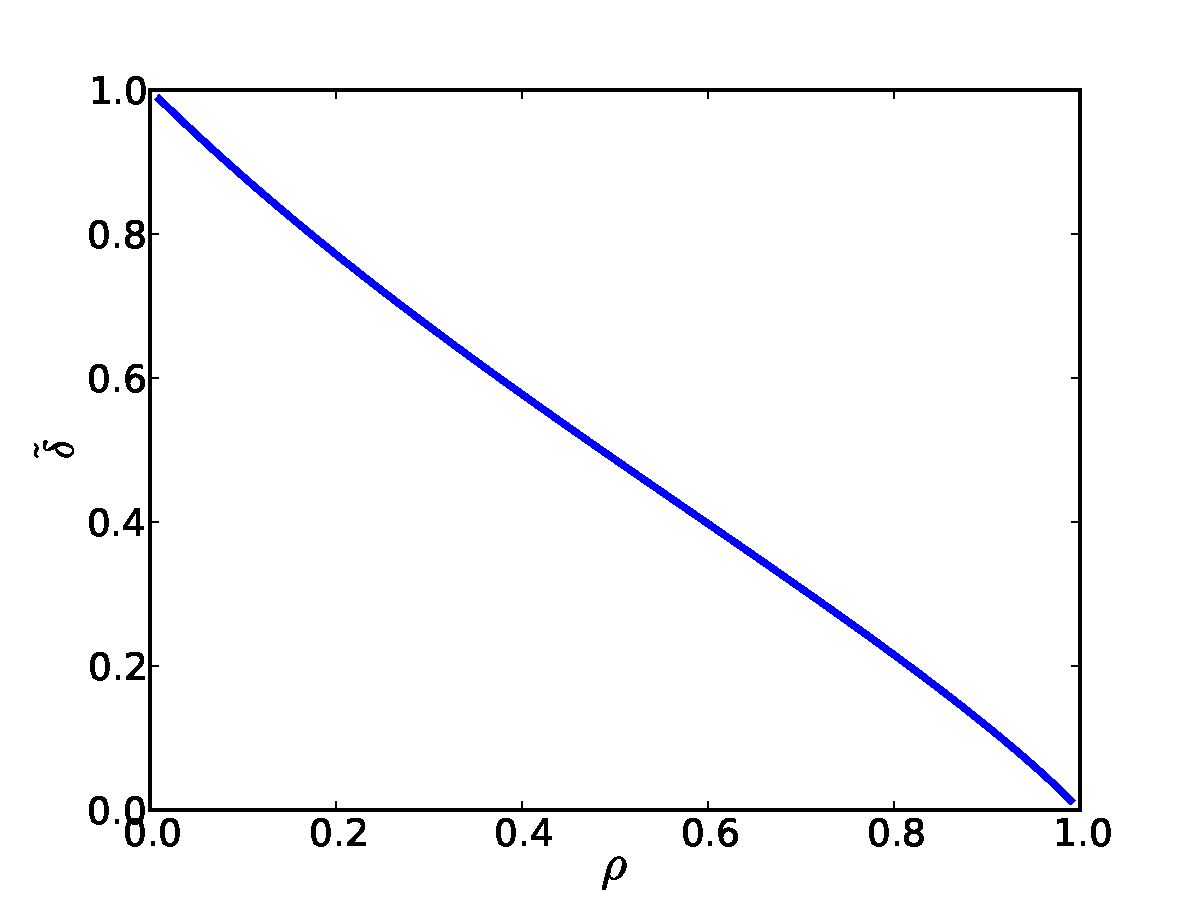
\includegraphics[width=0.7\textwidth]{Figures/delta-rho.pdf}
    \caption{Tendencia corroborativa efetiva $\tilde\delta$ em função do
    parâmetro de aprendizado $\rho$ da função de aprendizado Bayesiano.}
    \label{fig:delta-rho}
\end{figure}


%#}}}
